\documentclass{report}
\usepackage{graphicx} % Required for inserting images
\usepackage[italian]{babel}
\usepackage{tikz}
\usepackage{hyperref}
\usepackage{amsmath}
\usepackage{xcolor}
\usepackage{float}
\usepackage{soul}


\definecolor{darkgreen}{rgb}{0.0, 0.5, 0.0}


\title{Sistemi Multimodali}
\date{Parte XII}

\begin{document}

\maketitle

\tableofcontents
\newpage

\chapter{Sistemi Multimodali}

\section{Svantaggi dei sistemi monomodali}
\begin{itemize}
    \item Rumore dei dati in ingresso (illuminazione, umidità per le impronte, \dots)
    \item Variabilità intraclasse (posa nel volto, ferite su dita, raffreddore per la voce \dots)
    \item Limitata distintività del tratto biometrico (forma della mano, firma online, \dots)
    \item Non universalità del tratto
    \item Attacchi sul sensore
\end{itemize}

\section{Vantaggi e Svantaggi sei sistemi multimodali}

\begin{itemize}
    \item \textcolor{darkgreen}{\textbf{Vantaggi}}
    \begin{itemize}
        \item usare N tratti biometrici al posto di uno solo permette di aumentare 
        le performance di matching; sono più accurati
        \item si aumenta la copertura della popolazione riducendo il \textit{Failure to Enroll}
        
        $\rightarrow$ gli utenti che non possono registrarsi usando un tratto, possono usare gli altri
        \item sono un efficace metodo anti-spoofing; è molto più difficile ingannare contemporaneamente più sensori
    \end{itemize}
    \item \textcolor{red}{\textbf{Svantaggi}}
    \begin{itemize}
        \item sono più costosi essendo composti da più unità biometriche 
        \item sono più lenti in acquisizione, dato che occorre acquisire più tratti
    \end{itemize}
\end{itemize}

\section{Cosa si può unire?}
Multi-biometrico può signficare:
\begin{itemize}
    \item \textbf{Multiple biometrics:} \textit{volto e impronta digitale}
    \item \textbf{Multiple units:} \textit{indice destro e dito medio}
    \item \textbf{Multiple snapshots:} \textit{due template dell'indice destro}
    \item \textbf{Multiple matchers:} \textit{matching basato su minutiae e non-minutiae (metodi diversi)}
    \item \textbf{Multiple sensors:} \textit{sensori diversi}
\end{itemize}

\subsection{Quali tratti unire?}
Alcuni tratti sono spazialmente vicini (per esempio iride e volto) per 
\textbf{praticità di acquisizione}; altri sono distanti per garantire la 
\textbf{assoluta indipendenza dei tratti biometrici}.

\section{Applicazioni target}
Interesse potenziale per sistemi multimodali:
\begin{itemize}
    \sethlcolor{green}
    \item \hl{\textbf{Alto}}
    \begin{itemize}
        \item accesso fisico
        \item identificazione (documenti di identità elettronici)
        \begin{itemize}
            \item civile
            \item criminale
        \end{itemize}
    \end{itemize}
    \sethlcolor{yellow}
    \item \hl{\textbf{Moderato}}
    \begin{itemize}
        \item accesso a rete informatica o a terminale 
        \item chioschi informatizzati, sportelli ATM 
    \end{itemize}
    \sethlcolor{red}
    \item \hl{\textbf{Basso}}
    \begin{itemize}
        \item sorveglianza
        \item telefonia
        \item \dots
    \end{itemize}
\end{itemize}

\section{Terminologia usata in letteratura}
\begin{itemize}
    \item \textbf{Multimodale:} usa tratti biometrici scorrelati
    \item \textbf{Multiobiometrico:} cappello generale che comprende multimodale e sistemi 
    con tratti biometrici debolmente correlati, scorrelati, sensori diversi, software diversi, \dots
\end{itemize}


\chapter{Tecniche di datafusion biometrica}

\begin{figure}[H]
    \centering
    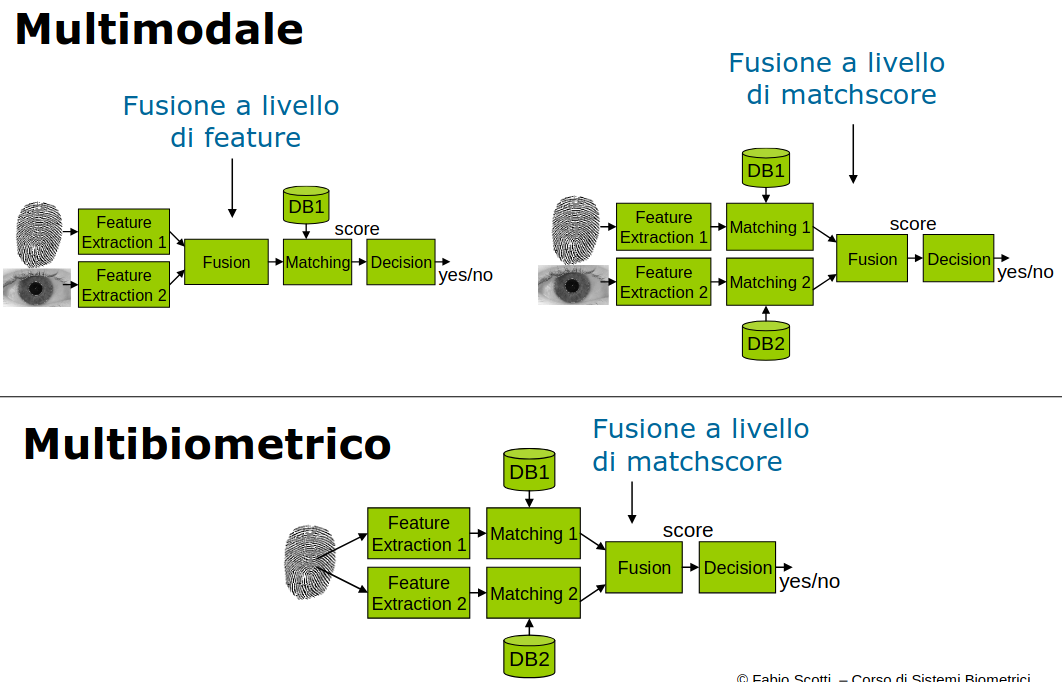
\includegraphics[width=1\linewidth]{images/schemi-fusion.png}
\end{figure}

\section{Normalizzazione degli score}
Per confrontare fra loro correttamente i valori di diversi 
matcher fra loro (valori di distanza tra template) è necessario eseguire 
prima una operazione di normalizzazione, per:
\begin{itemize}
    \item \textbf{omogeneizzare il significato} (ad esempio $s_1$ è una similarità 
    ed invece $s_2$ è una distanza)
    \item \textbf{riportare alla stessa scala} le uscite $s_1, s_2, \dots, s_n$
    \item \textbf{uniformare le distribuzioni} dei valori 
\end{itemize}

\noindent È sempre meglio tenere conto della:
\begin{itemize}
    \item \textbf{robustezza} (un valore molto diverso, magari provocato da un errore, non 
    deve stravolgere la normalizzazione)
    \item \textbf{efficienza} (occorre normalizzare avedo dei parametri stimati, vicini però a quelli reali)
\end{itemize}

\begin{figure}[H]
    \centering
    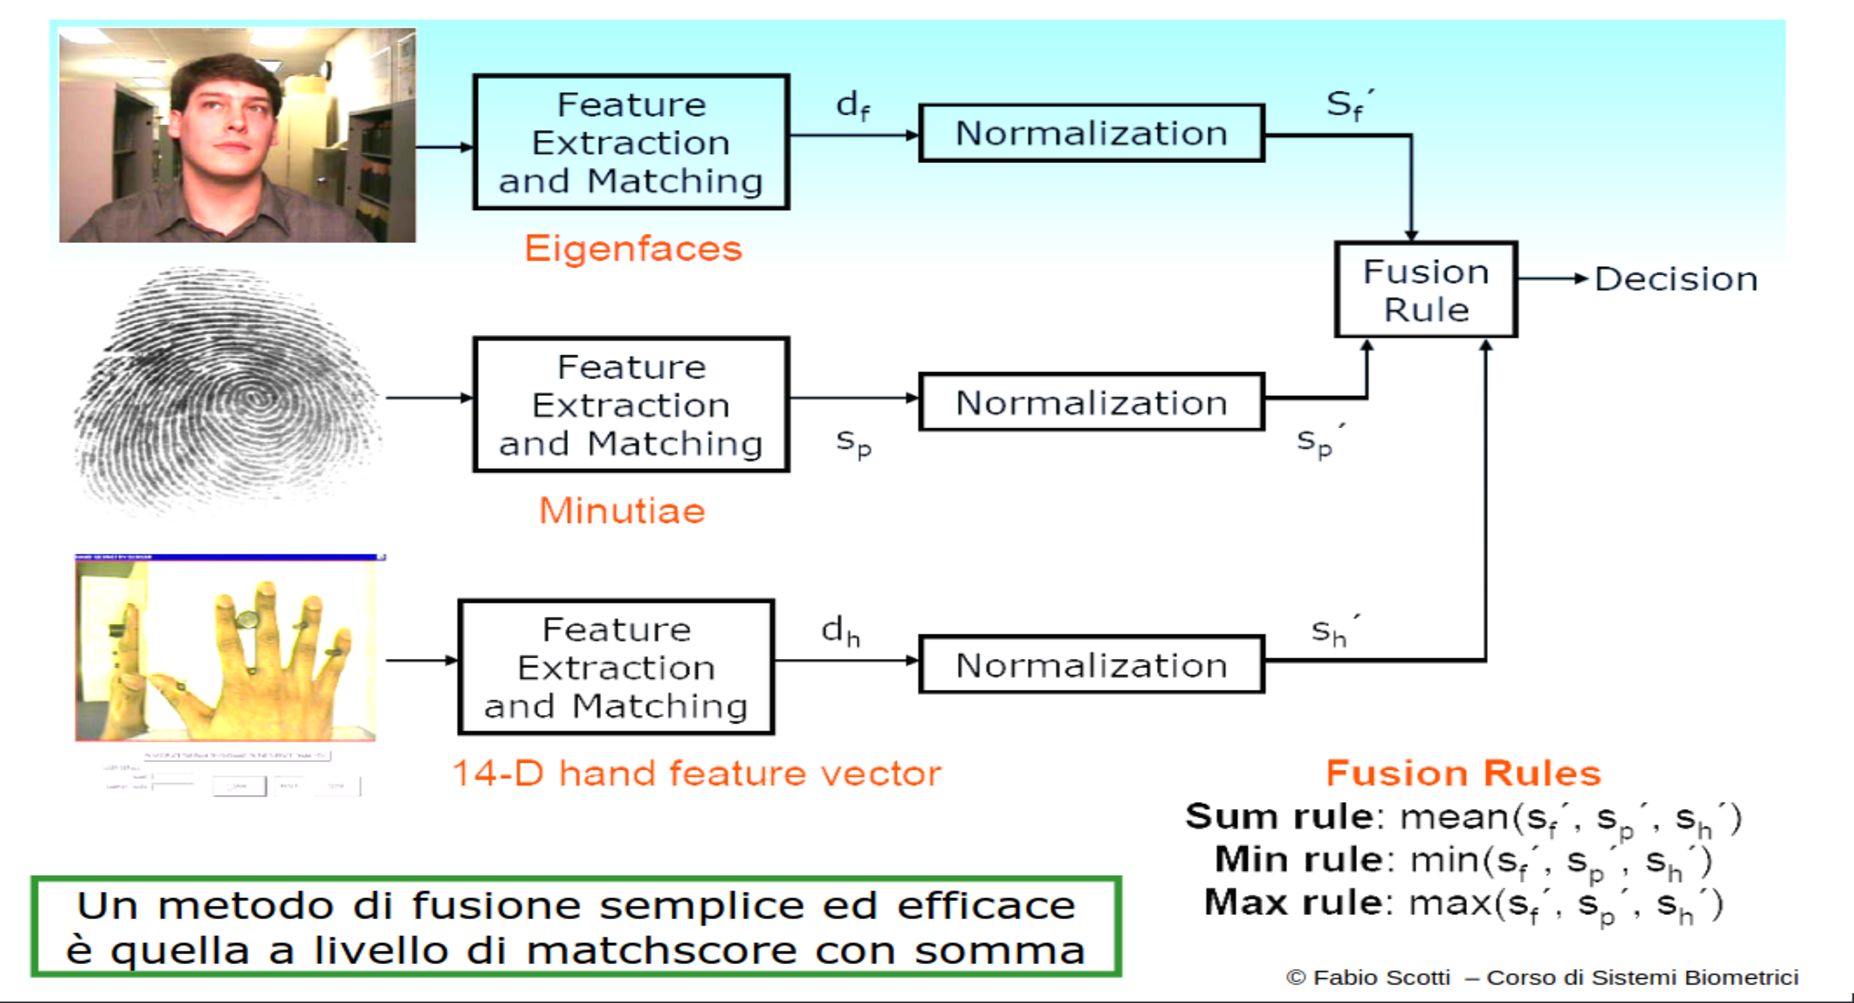
\includegraphics[width=1\linewidth]{images/fusion.png}
\end{figure}




\chapter{Tecniche avanzate di datafusion}

\section{Sistemi multimodali gerarchici}
Nei sistemi multimodali gerarchici \textbf{avvengono acquisizioni biometriche
in cascata a seconda del risultato dell'identificazione precedente}.
\begin{itemize}
    \item in \textbf{verification} riducono il tempo di verifica 
    \item in \textbf{identificazione} permettono mediante il \textit{pruning} di 
    ridurre le porzioni da analizzaree del DB (indexing)
    \item Per ridurre il tempo medio di verifica, \textbf{occorre acquisire per primi i 
    tratti biometrici più accurati}
    \item In certe applicazioni è l'utente che sceglie quale tratto mostrare
\end{itemize}


\section{Fusione a livello di feature}
Non è sempre facile riuscire a realizzare una efficace fusione delle informazioni 
a livello di feature. 

\noindent La principale causa è la \textbf{eccessiva eterogeneità fra le features};
di solito è possibile quando si estraggono da tutti i tratti biometrici delle 
\textbf{feature numeriche}.

\newpage
\section{Parametrizzazione specifica per \\ il singolo utente}
Esistono due approcci per aumentare ancora le prestazioni se viene tenuto conto delle carattersitche 
singolari di ogni utente:
\begin{itemize}
    \item ogni utente ha una \textbf{distanza dagli impostori personalizzata}
    \begin{itemize}
        \item ogni utente può quindi avere la sua \textbf{soglia di decisione personalizzata} per ogni tratto biometrico 
    \end{itemize}
    \item ogni utente produce delle acquisizioni biometriche dei tratti con \textbf{qualità diversa}; si possono 
    \textbf{pesare diversamente i tratti biometrici} tenendo conto:
    \begin{itemize}
        \item della qualità di acquisizione in enrollment per ogni utente 
        \item dell'errore di quel tratto biometrico (ad esempio, facciamo pesare di più le impronte 
        rispetto al volto nella decisione finale)
    \end{itemize}
\end{itemize}

\noindent$\rightarrow$ in altre parole, si hanno \textbf{due set di parametri} di progettazione
in un sistema biometrico multimodale: \textbf{le soglie dei matching e i loro pesi}

\section{Integrazione della soft biometrics}
Alcuni tratti chiamati \textit{soft biometrics} possono essere usati in aggiunta:
\begin{itemize}
    \item genere 
    \item colore della pelle 
    \item colore dei capelli 
    \item colore degli occhi 
    \item peso 
    \item altezza
    \item \dots
\end{itemize}

\noindent L'integrazione corretta di un sistema di soft-biometrics è a valle 
del modulo biometrico primario.


\chapter{Esempi di sistemi multimodali}

\section{Sistemi multimodali per il volto}
I sistemi innovativi per il riconoscimento del volto basati su \textit{multiple images}
o su \textit{2.5D faces} sono di fatto dei sistemi multibiometrici.

\noindent Grazie alla fusione delle informazioni sono riusciti a compiere un grosso 
passo in avanti.

\begin{figure}[H]
    \centering
    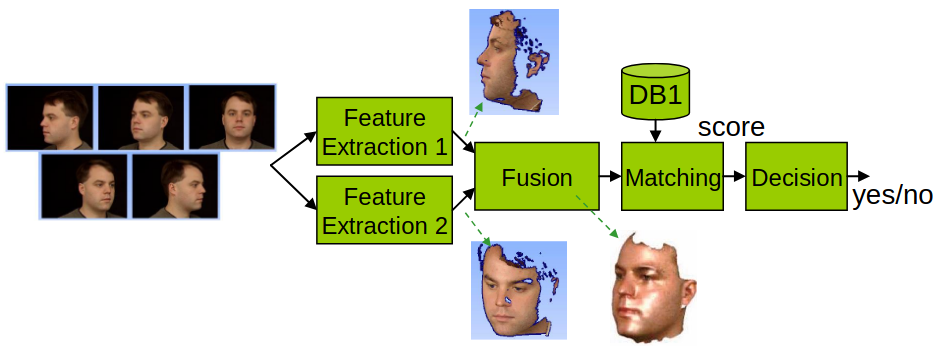
\includegraphics[width=1\linewidth]{images/volto.png}
\end{figure}

\section{Sistema BioID (parlato + volto)}
È un sistema che controlla:
\begin{itemize}
    \item riconoscimento del volto 
    \item sincronia fra il parlato e i movimenti delle labbra
\end{itemize}

\noindent Aumenta la robustezza del sistema contro gli attacchi.

\section{Sistema iride + retina}
Questo sistema implementa \textbf{due delle più accurate e resistenti 
agli attacchi tecnologie presenti sul mercato}. Ad oggi, è \textbf{impossibile
falsificare allo stesso tempo i due tratti}.

\begin{figure}[H]
    \centering
    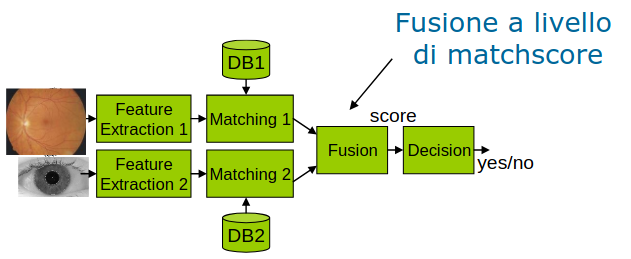
\includegraphics[width=1\linewidth]{images/iride-retina.png}
\end{figure}








\end{document}